\chapter{Methods, techniques, tools}\label{chapter:methods}
%\section{Introduction}\label{methods:intro}
This chapter introduces the representation of agents, swarms, obstacles, the environment, and the algorithms applied to inter-agent and obstacle interactions to produce a swarming effect. Movement of agents and the application of a \textit{destination vector} for goal based swarms are presented~\cite{MP:10}. 

\section{Modelling agents and swarms}
Currently, much swarm research uses field effects as the method of modelling inter-agent interactions~\cite{BAF:06, BAFVM:06, BM:09, APZDAMC:09, GP:02, GP:04, GP:04a, GP:05, GP:11, MYP:09}. The models usually use two field effects to implement the swarming characteristic. These effects are \textit{cohesion}, to draw agents closer, and \textit{repulsion} to prevent agents colliding. Field effects are the ranges around an agent that determine the effect other agents have upon its movement~(Figure~\ref{methods:FieldEffects}). It is usual for the cohesion field to have a radius $C_b$ which is larger than the repulsion radius $R_b$. When an agent ($b'$) moves into the \textit{neighbour field} of an agent ($b$) then $b'$ is said to be a neighbour of $b$ and is subject to cohesion. When an agent $b'$ moves into the repulsion field of $b$ then $b$ has a tendancy to move away from $b'$, i.e. to be repulsed. When an agent $b$ moves too close to an obstacle, i.e. within the obstacle repulsion range $O_b$, it has a tendancy to move away from the obstacle. 

A common approach to the application of field effects is to use fixed ranges common to all agents. Cohesion is applied graduated by neighbour proximity and repulsion is applied as a fixed magnitude when an agent is within the \textit{repulsion field}. 

Sensing devices have a limited range within which they detect agents, this determines a \textit{sensing field} shown is black~(Figure~\ref{methods:FieldEffects}). In a physical implementation of a swarm, distance may be determined by some form of sensing device such as an omni-directional camera, as used in the s-bot project~\cite{HR:ND,MFGAB:03,MIN:07}, or lidar~\cite{LJLYP:15} or ultrasonic sensors~\cite{BC:15} or by an array of simple proximity detectors~\cite{HWN:11}  

This thesis uses a similar approach to applying the cohesion effect but for repulsion a graduated field effect based on neighbour agent proximity is used.

\begin{figure}[H]
\begin{center}
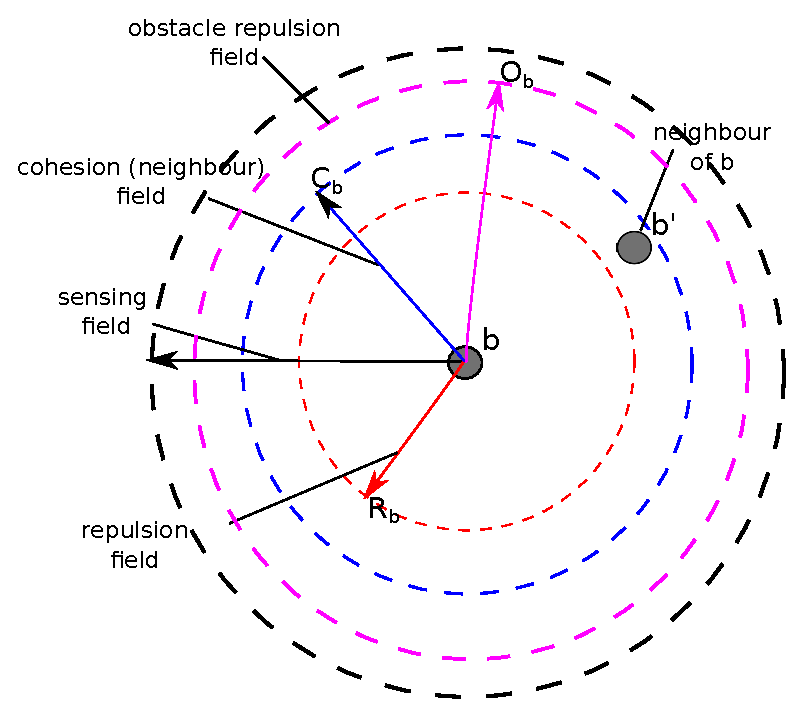
\includegraphics[width=7cm]{CHAPTER-2/figures/FieldEffects}
\end{center}
\caption{Agent field effects\label{methods:FieldEffects}}
\end{figure}

A swarm is modelled as a set of agents~\cite{MIN:07, VY:04}. An agent is modelled as a point in 2 dimensional space with no mass or size. This is similar to the representation used by Vankerkom and Yu to visualise swarms~\cite{VY:04}. Mohan and Ponnambalam, and Gazi and Passino~\cite{VY:04, GP:04}, Barnes et al.~\cite{BAF:06, BAFVM:06, BFV:07} and Bennet and McInnes~\cite{BM:09} and Andreou et al.~\cite{APZDAMC:09} also use a similar model which includes agents moving at a constant speed.

The interaction of agents within a swarm is modelled using vectorial and geometric techniques~\cite{HER:11, BAF:06}. The position of an agent is modelled using cartesian coordinates and the movements are modelled using vectors. The position vector is given by the coordinates of an agent.

The `world' that the swarm is modelled within is an unbounded 2 dimensional Euclidean plain.  

The use of vectors to model inter-agent interactions is also referred to a artificial potential fields~\cite{VG:05, XJYYH:10, SW:03, BAF:06, BAFVM:06, BFV:07, BM:09, HC:09} or vector fields~\cite{YH:14, GKF:13, PZ:13}. 
%% The mathematical techniques used to achieve the modelling are geometry and vector mathematics~\cite{HER:11, BAF:06}. The positional aspects of agents are modelled in the form of coordinate geometry and the movements are modelled using vector mathematics. These modelling techniques are highlighted in surveys carried out by Holmstr{\"o} and Romero~\cite{HR:ND}, Minor~\cite{MIN:07} and Muniganti and Pujol~\cite{MP:10}. 


%% Swarms can be modelled in two~\cite{MIN:07, VY:04} or three~\cite{BSB:15} dimensions.
%% This thesis uses a two dimensional model with unbounded ranges.%% \section{Swarming plane}
%% The modelling of swarms can be carried out in two dimensional planes. Swarms can be modelled in three dimensional space using the three axis of $x,y,z$~\cite{BSB:15} or two dimensional space using $x,y$~\cite{MIN:07, VY:04}.
%%  
%% This thesis uses a 2D Euclidean plane $(x,y)$. The dimensions of the plane are unlimited $(-\infty< x,y <+\infty)$ with a central origin of $(0,0)$. All the techniques discussed in this thesis could be transitioned to 3D space~\cite{PG:08} as a 2D environment can be considered as being a 3D environment with the $z$ axis set to $0$. 
                                
%% \section{Environment modelling principle}\label{method:RealNumberModelling}
%% Each agent's position within a swarm is modelled as a point consisting of two floating point numbers to represent their $(x,y)$ position.

\section{Modelling agents and environment interactions}\label{method:AgentEnvironmentModel}
The environment contains agents with a position in the coordinate system. It may also contain \textit{obstacles}~(Figure~\ref{section:ObstacleSection}) and \textit{destinations}~(Figure~\ref{sec:Direction1}). An obstacle can be considered as a point with an associated \textit{repulsion field} effect and a destination as a point towards which agents move. This modelling technique is similar to that used by Barnes et al.~\cite{BAF:06, BAFVM:06}. 
%% Modelling of the swarm will be performed using two techniques; vectors for inter-object interactions and coordinates for positional locations. The proximity of each of the objects within the swarm are identified, the objects being, agents, obstacles and destinations. The effects of the objects upon each other are determined using fixed ranges (field effects). 

The distribution of each of these objects, along with the field effects, produce sets of vectors that represent the inter-object interactions in the system. The vector sets for each agent are used to calculate a vector for each interaction type (cohesion, repulsion, direction, and obstacle repulsion). This is similar to the techniques used by Jung et al. and Salda\~na et al.~\cite{JG:13, SOM:12}. 

The resultant vector generated by an agent's interaction with other agents and obstacles is referred to as the agent's \textit{interaction vector}. The resultant vector generated between two agents is referred to as the \textit{inter-agent vector}. The vector applied to an agent to influence its movement towards a destination is referred to as the agent's \textit{destination vector}. The weighted combination of the \textit{destination vector} and the \textit{interaction vector} produces the \textit{movement-direction vector}. \textit{The movement-direction vector} indicates the direction an agent may move. 

%% \subsubsection{Swarming algorithms/model check} 
%% When calculating movement in a simulation the distance moved by the agents must be modelled in such a way that physically impossible scenarios do not occur. As agents are simulated mathematically it is possible for the simulation to calculate a path that would allow two agents to pass through the same space ($x,y$) at the same time. It is also possible to create environmental configurations that would allow an inter-object effect to be missed. This can be caused by the model not identifying agents passing through a field effect due to its calculated movement extending beyond or crossing a field effect in one time increment. 
%% These potential situations are eliminated by ensuring the sampling rate is a multiple of the clock cycle for calculating field effects, and the movement of an agent is less than any of the field effects. This check is incorporated into the simulator as a parameter check when the physics model of the graphical simulator is changed.

\section{Boid-based model}\label{methods:BoidModel}
The model introduced in~Figure~\ref{method:AgentEnvironmentModel} is based heavily on the work by Reynolds and other authors on boid-based swarms.

Hereford~\cite{HER:11} and Barnes et al.~\cite{BAF:06} model static swarms using a bi-variable technique. A bi-variable model is based upon inter-agent cohesion and repulsion, which appears as the \textit{interaction vector} above. 

Gazi and Passino also used this bi-variable technique to examine inter-agent interactions when creating stable swarm structures and ensuring agents remain part of a swarm while not colliding~\cite{GP:04a, GP:02, GP:04}. They define the degree to which an agent remains cohesive to a swarm as an agent's stability. 

If a swarm is to be goal based, the swarm is modelled using the \textit{interaction vector} and a \textit{destination vector} to create the \textit{movement-direction vector} as discussed by Salda\~na et al., Stranders et al., Nash and Koenig~\cite{SOM:12, SRDF:10, NK:10}. 

The first swarming model to use three components was the Boid model~\cite{REY:87}. In the Boid model, cohesion and repulsion are used to produce an \textit{inter-agent vector}. The main difference in the model is how the \textit{destination vector} is introduced. In a Boid swarm the \textit{destination vector} is not based upon a fixed destination. It is determined by each agent communicating with its neighbours to generate a consensus-based direction. Each agent calculates an average of the neighbours \textit{movement-direction vector} and applies the result as a \textit{destination vector}. This consensus-based movement creates a `flocking' effect~\cite{KC:08, REY:87}. This cooperative method of creating movement can be seen in the formation of fish shoals as discussed by Yang et al.~\cite{YGT:10} and Pearce et al.~\cite{PMRT:14}. The same flocking characteristic also occurs in starling murmurations as discussed by Campbell and Samsel~\cite{CS:15}, and Zhang et al.~\cite{ZZLW:14}. 

Barnes et al., Bennet and McInnes, Cai et al. Correl and Rus, Dinolov et al. and Ekanayake and Pathirana take a different approach to creating a \textit{destination vector}~\cite{BAF:06, BAFVM:06, BM:09, CML:ND, CR:13, DLK:11, EP:10}. They generate a \textit{destination vector} in a similar manner to that described in Figure~\ref{method:AgentEnvironmentModel} using the \textit{interaction vector} and the \textit{destination vector}.
%% The agent's position can be determined by using a sensor such as a GPS. The directional vector is added to the interaction vector. Adding the directional bias and the interaction vector produces a goal based characteristic in the resultant movement vector.
%% 
%% This thesis will use a similar method of generating a directional vector from a fixed destination to produce a \textit{Boid-based} directional model.  

\section{Swarm cohesion}\label{sec:Cohesion1}
Several views of cohesion exist within the swarm research community. Cohesion, in some cases, is considered as an agent moving towards the centroid of a swarm. The centroid is the centre of the swarm. This approach is used by Gazi and Passino who measure stability based on changes in distance from the centroid of a swarm~\cite{GP:11, GP:04}. They define stability as the `degree' to which a swarm will remain a coherent entity. Shinichi et al.~\cite{AYSH:08} also use the concept of the centroid of a swarm to define a metric to measure stability.

Alternatively Long et al.~\cite{QZYP:13}, Shinichi et al.~\cite{AYSH:08} and Ekanayake and Pathirana~\cite{EP:10} refer to cohesion as an `attractive force' and define cohesion as being localised to an agent and its `visible' neighbours. The visibility they discuss is determined by a sensor that provides localised proximity information that includes angles and distances to neighbouring agents.
 
Similarly, this thesis will view cohesion as the interaction of an agent with its local neighbours. Agents are viewed as being autonomous using only localised proximity information. The Boid model requires information about the swarm's structure, the positions and directions of neighbours. This requires a communications infrastructure. The model in this thesis does not require this information and therefore does not require a communications infrastructure.

This thesis, when analysing the data captured from an experiment, will only use the centroid as a means of tracking the position of a swarm. The centroid and the logic to identify it will not be used by agent algorithms for coordination. 

Cohesion is based on the principle that all agents will remain part of their immediate neighbours' `cluster' and will `flock' together in a `localised' manner~\cite{VGHHDM:15, BAF:06, BAFVM:06, BFV:07, BM:09, HAY:08, HCS:09}. Localised being that the agents will only be `aware' of their immediate neighbours. 

Flocking, in this thesis, should be considered as the process of agents moving towards each other to attain their most stable position~\cite{GMJ:11, IGMFM:08} which is the centre of mass of their immediate neighbours~(Figure~\ref{methods:FlyToCentre1}). 

The cohesion vector is calculated by summing the relative position vectors identified from the origin agent ($b$) to each neighbouring agent. This vector is divided by the total number of neighbour agents~(Figure~\ref{eq:FlyToCentre1}) to produce a resultant cohesion vector. The closer a neighbouring agent is to the agent of interest then the smaller the cohesion vector generated.

\begin{figure}[H]
\begin{center}
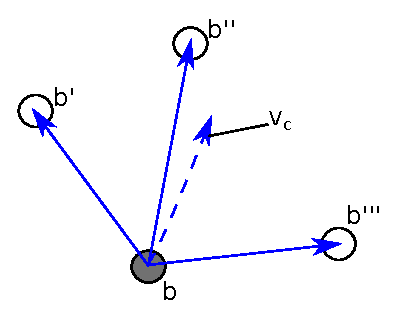
\includegraphics[width=5cm]{CHAPTER-2/figures/FlyToCentre1}
\end{center}
\caption{Cohesion: Origin $b$ \label{methods:FlyToCentre1}}
\end{figure}

Formally the cohesion vector $v_{c}(b)$ for agent $b$ is the vector calculated by summing the vectors $bb'$ formed from the agent to each of its neighbours~$b' \in nbr(b)$~\cite{HAY:08} and dividing by the number of neighbours.

%% $S$ is a swarm of size $N$ represented as a set of $N$ agents.
%% 
%% \begin{equation}\label{eq:Swarm1}
%% S \buildrel \Delta \over = \{b_{1}\ldots b_{N}\}
%% \end{equation}‎

A neighbour of $b$ is any agent within the swarm $S$ that is within neighbour range:

\begin{equation}\label{eq:Neighbours1}
nbr(b) \buildrel \Delta \over = \{b' \in S~:~\magn{bb'} <= C_b\}
\end{equation}‎

\begin{equation}\label{eq:FlyToCentre1}
v_{c}(b) = \frac{\mathlarger{\sum_{b' \in nbr(b)}}{bb'}}{\card{nbr(b)}}
\end{equation}‎

\section{Swarm repulsion}\label{sec:Repulsion1}
Repulsion is defined by Reynolds, Kawabayashi and Chen, and Shinichi et al. as the tendancy for an agent to move away from another agent that enters its repulson field~\cite{REY:87, KC:08, AYSH:08}. This creates a `field effect' around the agent such that when another agent enters that area a vector is applied to prevent the agents colliding. Repulsion is also applied to agents when they interact with obstacles, this is covered in~Figure~\ref{section:ObstacleSection}.

Kawabayashi and Chen~\cite{KC:08}, Reynolds~\cite{REY:87} and Aso et al. implement repulsion as a vector at a boundary with a fixed magnitude~(Figure~\ref{methods:Repulsion3}). 

\begin{figure}[H]
\begin{center}
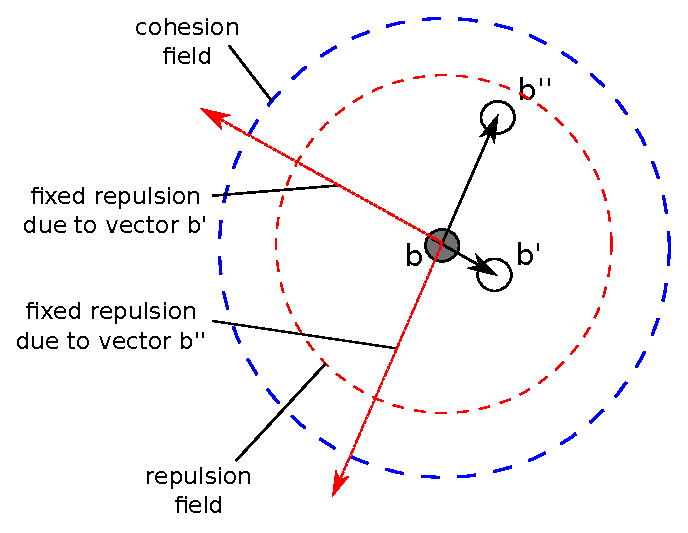
\includegraphics[width=7cm]{CHAPTER-2/figures/Repulsion3}
\caption{Agent fixed magnitude repulsion\label{methods:Repulsion3}}
\end{center}
\end{figure}

This approach produces a resultant repulsion vector that is based upon the angles at which the neighbour agents approach an agent without considering the proximity of the neighbours to the agent. 

In this thesis the repulsion vector has a graduated magnitude. Each neighbouring agent's repulsive effect is applied proportionally~(Figure~\ref{methods:Repulsion1}). When an agent encroaches upon another agent the degree of the field intrusion is mapped to a value in the range $0 \rightarrow 1$. This affects the magnitude of the repulsive vectors that are applied and therefore the resultant repulsion vector~(Figure~\ref{methods:Repulsion4}). 

\begin{figure}[H]
\begin{center}
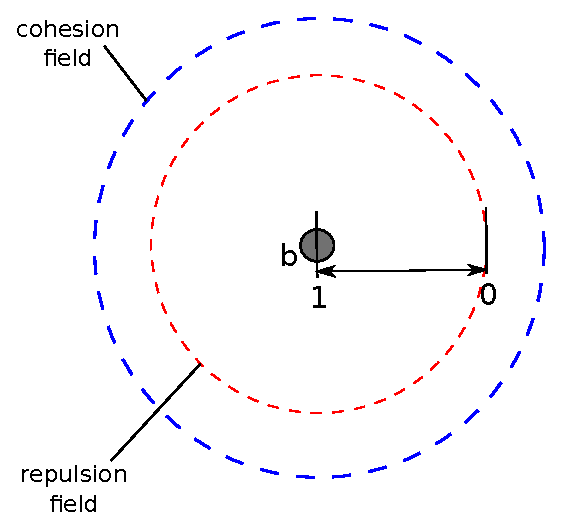
\includegraphics[width=8cm]{CHAPTER-2/figures/Repulsion1}
\caption{Graduated agent repulsion \label{methods:Repulsion1}}
\end{center}
\end{figure}

This technique changes the repulsion vector such that the direction reduces the probability of a collision. In this thesis the inter-agent repulsion will be calculated as the average of all the proportional repulsion vectors~(Figure~\ref{methods:Repulsion2}). 
 
\begin{figure}[H]
\begin{center}
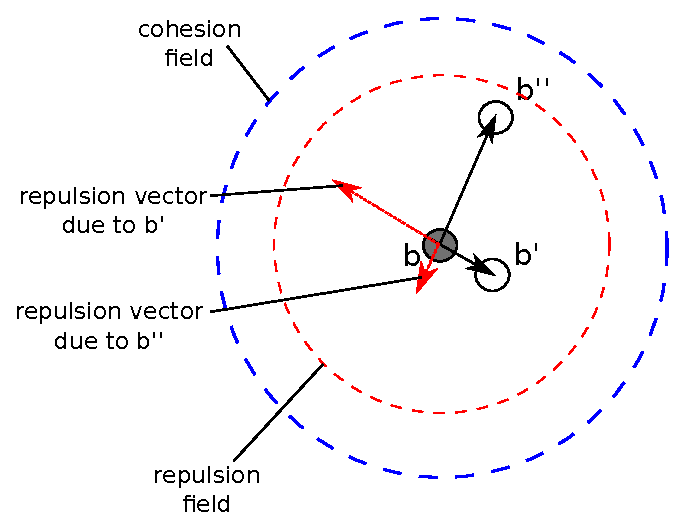
\includegraphics[width=7.5cm]{CHAPTER-2/figures/Repulsion2}
\caption{Proportional agent repulsion \label{methods:Repulsion2}}
\end{center}
\end{figure}

Figure~\ref{methods:Repulsion4} shows a comparison of the two repulsion models with the proportional repulsion magnitude shown in green and the fixed magnitude shown in red. The two models produce different repulsion angles. The angle produced by the proportional model increases the distance agent ($b$) will move away from $b'$ when motion is applied. This reduces the chance of a collision between the two agents. The proposed proportional model is therefore suited to swarm's where agent collisions may cause problems. 

\begin{figure}[H]
\begin{center}
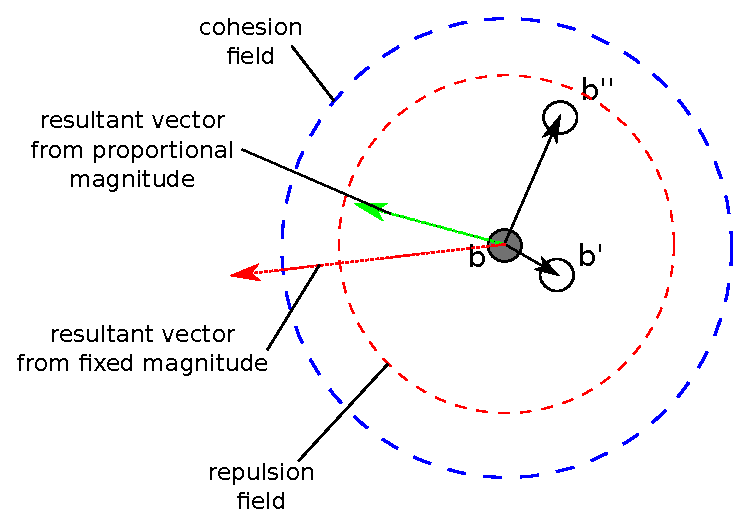
\includegraphics[width=8cm]{CHAPTER-2/figures/Repulsion4}
\caption{Repulsion comparison\label{methods:Repulsion4}}
\end{center}
\end{figure}

To calculate the total inter-agent repulsion the neighbours that are within the repulsion field must be identified. This is shown in~Figure~\ref{eq:Repulsion2}.

$R(b)$ is the set of all agents that are within the repulsion field. $R_b$ is the repulsion field and $\magn{bb'}$ is the distance between~$b$ and its neighbour~$b'$.  

\begin{equation}
\label{eq:Repulsion2}
R(b) = \{b' \in S~:~\magn{bb'} <= R_b\}
\end{equation}

$v_{r}(b)$ is the repulsion vector generated for agent $b$ based on the proximity of its neighbours. If $R(b)$ is empty then $v_{r}(b) = 0$ otherwise it is given by~equation~\ref{eq:Repulsion1}. The proportion of field intrusion is calculated by $1-\frac{\magn{bb'}}{R_b}$. The field effect distance $R_b$ is the range around the agent where the repulsion effect is introduced to prevent collisions. 

\begin{equation}
\label{eq:Repulsion1}
v_{r}(b) =‎ -
\frac{1}{\card{R(b)}}
\left(
\mathlarger{\mathlarger{\sum_{b' \in R(b)}}}
{\left( 1-\frac{\magn{bb'}}{R_b} \right)}
{bb'}
\right)
\end{equation}‎

\section{Swarm agents/obstacles interactions\label{section:ObstacleSection}}
Obstacles, like agents, can be represented as a point in the system. As an agent moves it may enter an obstacle's \textit{obstacle repulsion field} causing the agent to move away.

In this thesis agents are modelled with a fixed obstacle repulsion distance $O_b$ where a repulsion vector is applied. The repulsion is then a vector of magnitude $O_b$. If more than one obstacle is within the field effect agent the total repulsion vector is the sum of the repulsion vectors due to each obstacle~Figure~\ref{methods:Obstacle1}. The result is normalised and scaled such that the magnitude is the same as the field distance~$O_b$.

\begin{figure}[H]
\begin{center}
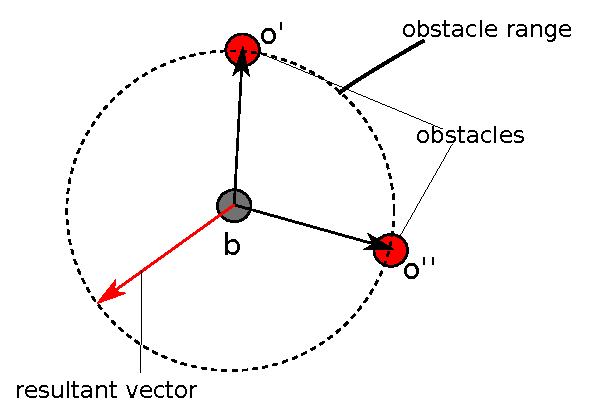
\includegraphics[width=6cm]{CHAPTER-2/figures/Obstacle1}
\end{center}
\caption{Obstacle repulsion \label{methods:Obstacle1}}
\end{figure}

%% $O$ is a set of $N$ obstacles.
%% 
%% \begin{center} \label{eq:Obstacle1}
%% \begin{equation}‎
%% O \buildrel \Delta \over =‎ \{o_1\ldots o_N\}
%% \end{equation}‎
%% \end{center}

%% $o' \in O:|bo'| < O_b$ the set of obstacles that are within range of agent $b$, where $O$ is the set of obstacles. 

%% \begin{center} \label{eq:Obstacle4}
%% \begin{equation}‎
%% R(b) \buildrel \Delta \over =‎ \{o' \in O:|bo'| < O_b\}
%% \end{equation}‎
%% \end{center}

Equation~\ref{eq:Obstacle2} shows the resultant repulsion vector $v_o(b)$ for an agent. $\{o~\in~O~:~\magn{bo}~<=~O_b\}$ is the set of obstacles that are within range of agent $b$. $O$ is the set of obstacles. The obstacles are identified using the distance between an agent and an obstacle $\magn{bo}$ and comparing the result to the fixed obstacle repulsion range~$O_b$. The result is calculated by scaling the normalised sum of the normalised vectors $(ob)\string^$ by $O_b$. Note that \string^ is the equivalent of $\hat{v} = \frac{v}{\magn{v}}$ the normalised vector.

\begin{center} 
\begin{equation}\label{eq:Obstacle2}‎
v_o(b) =‎ O_b\Bigg(\mathlarger{\mathlarger{\mathlarger{\sum}}}_{o \in O~:~\magn{ob} <= O_b}(ob)\string^\Bigg)\string^
\end{equation}‎
\end{center}

%% \begin{center} \label{eq:Obstacle3}
%% \begin{equation}‎
%% v_o(b) =‎ |l_o(b)|O_b
%% \end{equation}‎
%% \end{center}

\section{Swarm direction (goal based swarms)}\label{sec:Direction1}
There are two directional aspects to swarm motion. The \textit{interaction vector} which is the vector created by inter-agent reactions through the cohesive and repulsive fields as discussed in~Figure~\ref{sec:Cohesion1} and~Figure~\ref{sec:Repulsion1} and the vector for avoidance of obstacles~Figure~\ref{section:ObstacleSection}. The \textit{destination vector} is applied to influence the motion of a agent towards a particular coordinate~\cite{BHK:07} and the \textit{interaction vector} to maintain the swarm's structure. This model is used by Barnes et al.~\cite{BAF:06, BAFVM:06}, Bennet and McInnes~\cite{BM:09}, Cai et al.~\cite{CML:ND}, Correll and Rus~\cite{CR:13}, Dinolov et al.~\cite{DLK:11} and Ekanayake et al.~\cite{EP:10}. This thesis uses a similar technique, defining a single destination as a \textit{destination vector} for goal based swarms. The application and effect of multiple destinations is discussed in future work. 

%% \begin{figure}[H]
%% \begin{center}
%% \includegraphics[width=7cm]{CHAPTER-2/figures/Destination1}
%% \caption{Destination vector\label{methods:Destination1}}
%% \end{center}
%% \end{figure}

$v_d(b)$~(Equation~\ref{eq:Destination1}) is the \textit{destination vector} where $d$ is the destination. 

\begin{center}
\begin{equation}\label{eq:Destination1}‎
v_{d}(b) =‎ bd
\end{equation}‎
\end{center}

\section{Weighted movement-direction model}\label{methods:weightedModel}
An agent's \textit{movement-destination vector} is the sum of all the component vectors ($v_c, v_r, v_d, v_o$) (Equation~\ref{eq:BotDirection1})~\cite{HAY:08}. For a vector to be used for movement it must have a magnitude of 1 before the agent's speed can be applied (Section~\ref{sec:Direction1}).

%%  as shown in~(\autoref{eq:BotDirection1}).
 
\begin{center}
\begin{equation}
\label{eq:BotDirection1}
v(b) =‎ v_{c}(b) + v_{r}(b) + v_{d}(b) + v_{o}(b)
\end{equation}‎
\end{center}

%% Note: \string^ is the equivalent of $\hat{v} = \frac{v}{|v|}$ the normalised vector.

This model is extended by adding a weighting to each of the component vectors. The addition of the weightings allows the influence of each component vector set to be adjusted to produce a bespoke movement vector~(\autoref{methods:weightedModel}). The resultant vector is normalised to produce a unit \textit{movement-direction vector} that can be used to create motion~\cite{KC:08}. The agent's speed characteristic is used along with time~($t$)~\cite{FAP:05, GP:05} to determine an agent's next position. This derived vector is the \textit{movement vector}.

The purpose of a weighted aggregation model is to alter the level of influence of each component of the equation. This technique is generally referred to as a \textit{`weighted sum aggregation'} or \textit{`ordered weighted averaging'}. The technique is applied to optimisation algorithms such as PSO (Particle Swarm Optimisation) and involves applying all the possible combinations of weightings to a multi-variable expression to obtain an optimum output~\cite{MV:12, XTH:09}.

In this thesis the technique of \textit{weighted sum aggregation} is applied to the vector calculations to allow tuning of the swarming algorithm of an agent and to change the degree of influence to obtain a required swarming effect. 

The tuning is applied to each component as a weighing factor $k$~Equation~\ref{eq:BotPhysics1}. The weightings ($k_c, k_r, k_d, k_o$) are applied before normalising the \textit{movement-directional vector}. This change of bias allows levels of importance to be applied to a system characteristic i.e. $k_c > k_d$ implies it is more important for the agents to remain together than it is to travel towards the destination. This technique is similar to those identified by Muniganti and Pujol in their survey of mathematical modelling techniques~\cite{MP:10}. 

Weightings can be applied in several ways. The weighting can be applied as a set of arbitrary integer values (12, 67, 99) or as a set of values that always have a summed value of 1 e.g. 0.5, 0.25, 0.25. Either of these techniques are acceptable as the resultant vector is normalised following the application of the weighting. This thesis implements the weightings as a set of arbitrary integer values~(Equation~\ref{eq:BotPhysics1}). Where $k_c$ is the weighting factor for cohesion, $k_r$ is the weighting factor for repulsion, $k_o$ is the weighting factor for obstacles and $k_d$ is the weighting factor for a destination. 

\begin{equation}\label{eq:BotPhysics1}‎
v(b) =‎ k_cv_c(b) + k_rv_r(b) + k_ov_o(b) + k_dv_d(b)
\end{equation}‎

Special cases of~Equation~\ref{eq:BotPhysics1} can be applied to a swarm model. A swarm with no destination can be modelled with the destination weighting set to zero to create the model shown in~Equation~\ref{eq:BotDirection2} as used in Chapter~\ref{chapter:flooding}. This is also known as the \textit{interaction vector}

\begin{center}
\begin{equation}
\label{eq:BotDirection2}
v(b) =‎ k_cv_c(b) + k_rv_r(b) + k_ov_o(b)
\end{equation}‎
\end{center}

A swarm that does not interact with obstacles and has no goal (destination) can have $k_o$ and $k_d$ set to zero creating the model as shown in~Equation~\ref{eq:BotDirection3}. This is also known as the \textit{inter-agent vector} as discussed in~\autoref{Section:StabilityModel} on page \pageref{Section:StabilityModel}.

\begin{center}
\begin{equation}
\label{eq:BotDirection3}
v(b) =‎ k_cv_c(b) + k_rv_r(b)
\end{equation}‎
\end{center}

Equation~\ref{eq:BotDirection3} is also the model used in the calculation of the swarm magnitude metric as discussed in chapter~\ref{chapter:metric} where $v(b) \equiv P(b)$.

\section{Modelling movement}\label{sec:Movement1}
Each agent within a swarm calculates its \textit{movement-direction vector} based on its \textit{interaction} and \textit{destination} vectors. The \textit{movement vector}~($b_{pos}$) is calculated using the unit \textit{movement-direction vector} of Equation~\ref{eq:BotPhysics1} multiplied by the time elapsed~($t$) in the system and the speed characteristic of the agent~($s_b$).

This process is carried out for every agent in the swarm to create the entire swarm's next position.

\begin{center}
\begin{equation}
\label{eq:AgentMovement}
b_{pos}=s_{b}t\big(v(b)\big)\string^ 
\end{equation}‎
\end{center}

The increment in the location of agent $b$ over time interval $t$ is shown in Equation~\ref{eq:AgentMovement} where $s_b$ is the speed of agent~$b$. Models of time are discussed in chapter~\ref{chapter:simulator}. 

%% \begin{center}
%% \begin{equation}
%% \label{eq:BotSwarm2}
%% l(b) =‎ s_{b}t\big(v(b)\big)\string^
%% \end{equation}‎
%% \end{center}



%% \section{Swarming algorithms} 
%% The logic that produces the cooperative appearance of agents in a swarm are the algorithms that each agent applies to calculating their movement~\cite{BS:13, DLK:11, HAY:08}. There are many variation in how algorithms apply their effects~\cite{BBBV:04, DT:03}. The basis of all algorithms is that they consider two influencing factors, direction and speed~\cite{BAF:06, BAFVM:06, BVD:14, EP:10}. 
%% 
%% The application of the movement is therefore calculated using the time, speed and direction in discrete intervals as shown in~\autoref{method:SwarmParticipant} where $s_b$ is the agent speed, $t$ is time, $b$ is the agent and $v$ is the resultant vector that is used to calculate the movement.
%% 
%% \begin{figure}[H]
%% \begin{center}
%% \includegraphics[width=7cm]{CHAPTER-2/figures/SwarmParticipant}
%% \caption{Algorithm effects \label{method:SwarmParticipant}}
%% \end{center}
%% \end{figure}

\section{Stable swarm structures}
A swarming behaviour can be created using only cohesion and repulsion. This technique is known as a bi-variable model~\cite{BAF:06,BAFVM:06}. The bi-variable model produces natural geometric structures. The structures tend to be based on equilateral triangles and when the distribution of the agents allows, regular hexagons are formed. These structures only occur when the repulsion and cohesion field effects produce a distribution such that an agent's detected neighbours do not extend beyond the first agent detected in any direction~\cite{PCL:08, PCL:08a}. The effect of field effect ranges on a swarm's structure is discussed in chapter~\ref{chapter:SwarmType}.  

The most stable state for agents is for all agents to be equidistant with equal angles. If two agents are in close proximity they will naturally adhere to each other due to the proximity rule (cohesion)~(Figure~\ref{fig:StableForms}); repulsion will ensure a minimum distance is preserved. In the case of 3 agents a triangle will form. In the case of 4 agents the most stable shape will be a diamond with the centre agents joined. With 5 and 6 agents a triangular lattice will emerge and with 7 agents a stable hexagon will form. The hexagon~(Figure~\ref{fig:StableFormHexagon}) is the most stable structure with all agents being equidistant and all angles between each neighbouring agent equal~\cite{BAF:06, GP:05}. These structures are seen throughout the natural world~\cite{RAZ:13}.

\begin{figure}[H]
\begin{center}
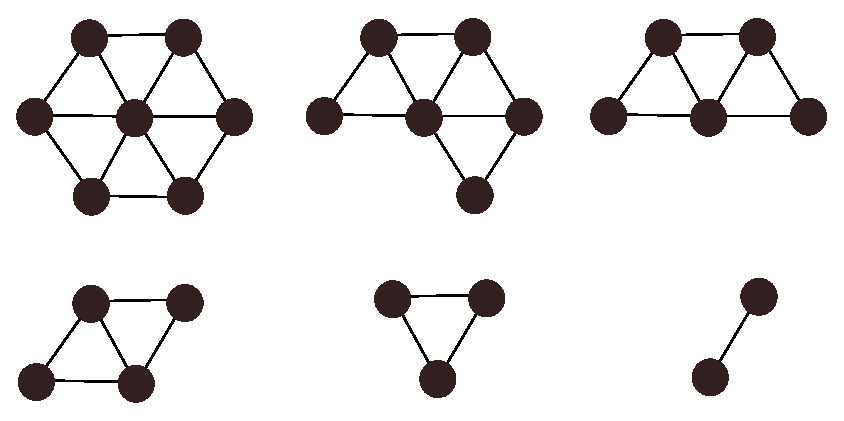
\includegraphics[width=7cm]{CHAPTER-2/figures/StableForms}
\end{center}
\caption{Stable swarm formations}\label{fig:StableForms}
\end{figure}

\begin{figure}[H]
\begin{center}
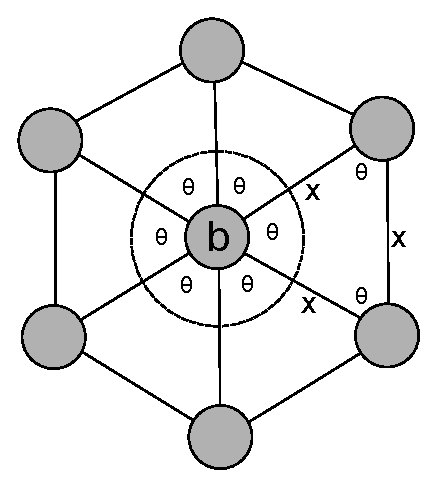
\includegraphics[width=4cm]{CHAPTER-2/figures/Hexagon}
\end{center}
\caption{Stable hexagonal formation}\label{fig:StableFormHexagon}
\end{figure}



\section{Resultant swarm model}
The swarm model created by~Equation~\ref{eq:BotPhysics1} with suitable weightings will allow a swarm to form `stable' structures such that the agents will remain connected~(\autoref{methods:Stable1}) and over time migrate to an optimum overall structure for the models parameters. The parameters are the field effect ranges, the cohesion and repulsion magnitude models and the weightings. 

The initial random deployment of a set of agents to create a swarm produces a `disorganised' state. The disorganisation is caused by the varying cohesion and repulsion vectors that are generated by the inter-agent relationships. Following the initial deployment the magnitudes will create movements that gradually stabilise the swarm structure to a level of movement that best fits the model parameters~\cite{PG:08, WF:12}. The point of equilibrium for the swarm and the resultant structure is dependant upon the agent's cohesion and repulsion fields level of overlapping. This is discussed in \autoref{section:AnalysisA} and~\autoref{section:AnalysisB}.

When modelling swarms it is common practice to have the agents in constant motion~\cite{LCW:07, GKF:13}. In this thesis agents are modelled moving at a constant speed with no inertial effect such that an agent can move freely within the system plane. The only exception to this will be if an equilibrium state is encountered where the summed vectors produce a null vector. If this occurs the agent will stop moving.

\section{Swarm deployment}

Using the methods discussed in this chapter, a swarming behaviour emerges from
a collection of agents. The initial deployment of a swarm may be a random
dispersal of agents such that the swarm is in a disorganised
state~(\ref{methods:Chaos1}), caused by an instability in the magnitudes that
are acting upon each of the agents (as detailed above). Based upon the
application of the models discussed, the swarm will initially move in such a
way as to balance all the vectors, resulting in a period of disorganisation
where the swarm's movement towards a goal is limited, as the vectors generated
to disperse the agents outweigh the directional vector. 

This phase of the swarm's life cycle is the `initialisation
phase'~(Figure~\ref{methods:StableTime1}). When the initialisation phase is
over, the vectors (cohesion, repulsion, and direction) become more balanced and
the swarm forms a more regular shape, such as a hexagonal lattice, where all
the angles and lengths (distances between agents) tend toward being
equal~(Figure~\ref{methods:Stable1})

The effects can be seem in the screenshots (Figures \ref{methods:Chaos1},
\ref{methods:Stable1}, \ref{methods:StableTime1}) from the simulator discussed
in section~\ref{chapter:simulator}.

\begin{figure}[H]
\begin{center}
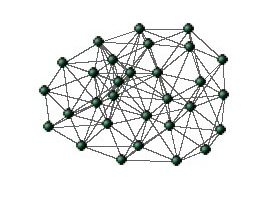
\includegraphics[width=7cm]{CHAPTER-2/figures/Chaos}
\end{center}
\caption{Disorganised swarm\label{methods:Chaos1}}
\end{figure}

\begin{figure}[H]
\begin{center}
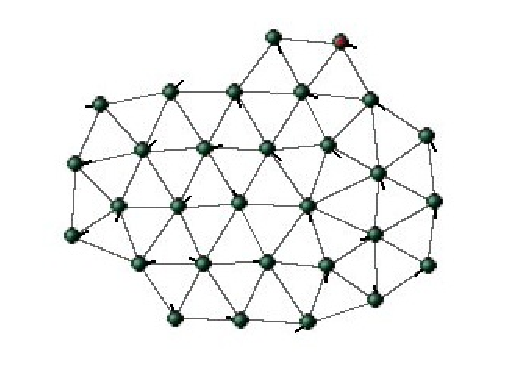
\includegraphics[width=7cm]{CHAPTER-2/figures/Stable}
\end{center}
\caption{Stable swarm\label{methods:Stable1}}
\end{figure}

\begin{figure}[H]
\begin{center}
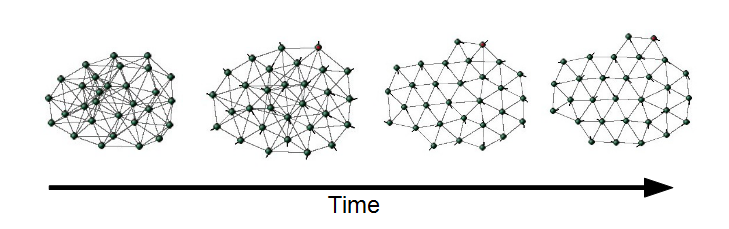
\includegraphics[width=10cm]{CHAPTER-2/figures/StableTime}
\end{center}
\caption{Swarm stabilisation\label{methods:StableTime1}}
\end{figure}

\section{Swarm simulator}\label{chapter:simulator}
Swarm behaviours can be investigated by means of experiments with physical robots or by means of simulations. The latter approach has the advantages of scalability, genralisation, speed of development, and cost. This thesis is based upon data generated from simulated swarms. There are several open source robotic simulators available, the most popular being ARGoS, Player/Stage, and Gazebo.

ARGoS is described as a multi-physics simulator and has gained interest in the swarm robots community. In 2011 Luca and Caro published an overview of the simulator's engine discussing how the system functioned~\cite{PTOPB:11} and the philosophy behind its structure. They also published a framework for using the simulator in 2012~\cite{KCGD:12}. 

Player/Stage and Player/Gazebo are used in many projects including projects simulating single robots as discussed by Song and Gupta~\cite{SG:15} and also multiple-robot swarming simulations as decribed by Lei et al~\cite{LLZ:08}. There are projects that have simulated the use of pheromone trails when simulating foraging based swarms as discussed by Shi et al~\cite{STZZW:13}. Shi et al. have also published an overview of the scenarios in which Player/Stage can be used~\cite{STWZZ:11}.

The Webot~\cite{CL:16} simulator, which is a commercal product, has been used successfully in other research projects such as the swarm simulations developed by Srivastava and Nandi~\cite{SN:10}. One problem found with the product was that it was restrictive in terms of how much of the system could be configured to meet the needs of the thesis. Another factor that had to be taken into consideration was the high cost of a licence for the PRO version of Webot.

These simulators all provide a discrete time simulation environment. The main purpose of these simulators is to visualise either an individual robot or a swarm of robots based on a model that is defined through bespoke libraries and configuration parameters. On the other hand, in this thesis the main purpose of each simulation is to log all the positional and vector data associated with every agent at each discrete time interval. Due to this disparity in approaches it was decided to develop a simulator whose main purpose is the collection of data on distance, positions, distribution and inter-object vector magnitude influence. 

This section discusses the design, development and usage of the simulator used in this thesis and the creation of the raw experimental data. The section also discusses how the data is processed to produce the aggregated data required for visualisation.

%\section{Introduction}\label{sim:intro}

\subsection{Development overview}\label{sim:intro}
The simulator has two distinct components: a graphical design/simulation tool~(Appendix~\ref{AP2:GRAPH}) and a command line based simulation-only tool~(Appendix~\ref{AP2:CLI}). Both parts of the simulator are written in Python 3~\cite{PYTHON3:15} using an object model as shown in~appendix~\ref{app5}. Both use the same modelling engine by sharing the base classes.  The final object model is similar to that proposed by Vankerkom and Yu for swarm visualisation~\cite{VY:04}. The simulator design is also influenced by the \textit{`main loop'} proposed in the ARGoS simulator~\cite{PTOPB:11}.

\subsection{Swarm simulator software}\label{sim:Simulator2}
The main purpose of the graphical environment is for the setup of an experiment's initial configuration. This is achieved by positioning the agents, destinations, and obstacles in an environment and saving the configuration as a simulation file. As a secondary purpose the graphical environment is capable of running small scale simulations. The command line tool is used to execute the simulation experiments designed using the graphical tool. 

The graphical tool, shown as (1) in~Figure~\ref{sim:SimulatorOverview}, uses PyGame~\cite{PYGAME:15} as its graphical presentation layer. PyGame supports several rendering engines; in this application the default SDL rendering engine is used. The graphical simulator runs in real-time and is capable of simulating small swarms of \textless~150 agents on a PC with an \texttt{Intel® Core™ i7-4770 CPU @ 3.40GHz * 8} processor. This swarm size limitation is due to the Python code being executed on a single processor core. There is also a limitation in the performance of the graphical engine due to the rendering being performed by the interpreter.
 
The command line tool, shown as (2) in~Figure~\ref{sim:SimulatorOverview}, reads in the experiment configuration file generated via the graphical tool, shown as (1). The command line tool uses simulated descrete time~(Figure~\ref{sim:time}) and is able to run with arbitrary sized swarms without real-time processing limitations. The command line tool simulates the swarm and generates the initial data extract (3a). The data extract is then loaded into a MySQL database (3b) and the data is then agregated to create the complete dataset for the experiment (4). The processes 5 and 6 are discussed in~Figure~\ref{sim:GraphingTools}.  This thesis deals with arbitrary sized swarms, so simulations are designed in the graphical environment but executed using the command-line-based simulator. 

\begin{figure}[H]
\begin{center}
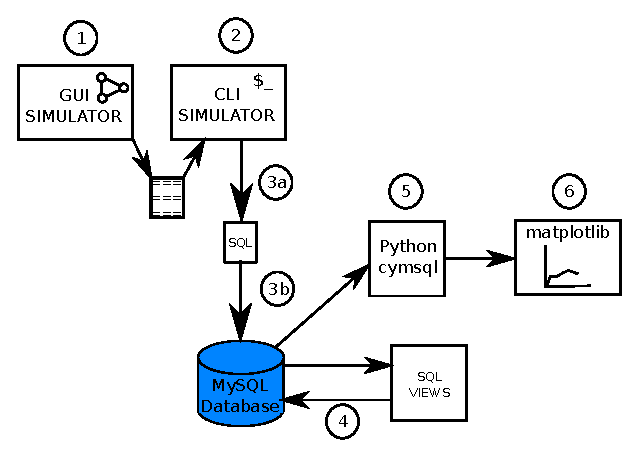
\includegraphics[width=10cm]{CHAPTER-3/figures/SimulatorProcess}
\end{center}
\caption{Simulator process overview\label{sim:SimulatorOverview}}
\end{figure}

Figure~\ref{sim:SimulatorOverview} shows the stages of the simulation from developing an experiment~(1) through to the production of simulation results~(6).

\subsection{Motion modelling implementation}
The motion model of the simulation is implemented through the modelling of vectors that influence an agent's resultant direction. The vectors that model the swarm environment are the cohesion and repulsion vectors created by inter-agent and inter-object interactions. 

Agent positions are modelled using floating point numbers. These coordinates are translated to integer based $(x,y)$ co-ordinates for the presentation layer. The integer translation is only for the visualisation of the swarm. This is the same approach used by Vankerkom and Yu in their paper on swarm visualisation~\cite{VY:04}. They model the agent using a class that consists of positional variables of type double. This is also seen in the SwarmVis software developed by Miner and Kasch~\cite{DMNK:ND}.

\subsubsection{Modelling Time}\label{sim:time}
There are two options for representing time when modelling a swarm: continuous time and discrete time. Continuous time~\cite{HW:08} is \textit{dense}: between any two points in time there is another point. Discrete time~\cite{FAP:05, GP:05, RVMH:13, HER:11, MP:10, PCL:08a} on the other hand proceeds in `ticks' with no intermediate time points. In this thesis discrete time is used. This same approach is identified by Muniganti and Pujol in their survey of mathematical swarming models~\cite{MP:10}. 

\subsubsection{Sensor modelling}
Vision based coordination for robots was a subject of great interest in the 1980s and 90s~\cite{DK:02}. This interest moved to omni-directional cameras as a means of determine position and mapping through image analysis in a process known as SLAM (Simultanious Localisation And Mapping)~\cite{TRI:15,SG:15}. A general purpose omni-directional camera can operate at speeds between 1Hz and 60Hz depending upon the resolution of the images and the accuracy of the positional data required. In simulations in this thesis an operating speed of 10Hz (100ms) will be used. 

For the identification of an agent's position a GPS with a sample rate of the same speed may be used. Using these two sensors would allow for positional and location based informtion to be available every 100ms. Faster update rates for GPS sensors are available such as the SparkFun Venus GPS~\cite{SF:16} which operates at up to 20Hz. For the modelling experiments in this thesis 100ms is sufficient.

\subsubsection{Cohesion implementation}
Within the simulation the neighbour range is calculated by comparing a set distance (neighbour range) to the magnitude of the \textit{inter-agent vectors}.

An agent's cohesion is implemented in the simulation software as~Listing~\ref{code:cohesion1}. Line~\ref{line:neighbours} shows the iteration over all the neighbours. Line~\ref{line:sumVectors} calculates the sum of the vectors created by the neighbours. Line~\ref{line:resultantCohesion} divides the summed vectors by the number of neighbours. This process generates the cohesion vector for an agent to its neighbours.

\lstset{language=Python,
basicstyle=\tiny,
numbers=left, 
numberstyle=\tiny,
captionpos=b,
frame=single,
breaklines=true,
caption=Cohesion code,
escapechar=|
} % Set your language (you can change the language for each code-block optionally)
\begin{lstlisting}[label={code:cohesion1}]  % Start your code-block

def flyTowardsCentre(participant):
  newVector = Vector2()
  if len(participant.neighbours):
|\label{line:neighbours}|  for bot in participant.neighbours:
|\label{line:sumVectors}|    newVector += Vector2(bot.x,bot.y)
|\label{line:resultantCohesion}|    newVector = (Vector2(newVector.x / len(participant.neighbours),newVector.y / len(participant.neighbours)) - Vector2.from_floats(participant.x,participant.y))
  return newVector
\end{lstlisting}

\subsubsection{Repulsion implementation}
Listing~\ref{code:repulsion1} shows the implementation of inter-agent repulsion in the simulation software. This effect reduces the possibility of agents colliding. Line~\ref{line:calcDistance} identifies the distance between a neighbour and an agent. This distance is then used to identify if a repulsive vector needs to be generated (Line~\ref{line:isRepulsion}). Lines~\ref{line:amountRepulsion} and~\ref{line:applyRepulsion} calculate the proportional effect of the repulsion that is then applied to an agent.

\lstset{language=Python,
basicstyle=\tiny,
numbers=left, 
numberstyle=\tiny,
captionpos=b,
frame=single,
breaklines=true,
caption=Repulsion code,
escapechar=|
} % Set your language (you can change the language for each code-block optionally)
\begin{lstlisting}[label={code:repulsion1}]  % Start your code-block

def moveAway(participant):
  newVector = Vector2()
  for bot in participant.neighbours:
|\label{line:calcDistance}|    distanceVector = Vector2.from_points((bot.x,bot.y),(participant.x,participant.y))
    distance = distanceVector.get_length()
|\label{line:isRepulsion}|    if participant.minimumClearDistance > distance and distance > 0:
|\label{line:amountRepulsion}|      percentagePush = ((participant.minimumClearDistance - distance) / distance)
|\label{line:applyRepulsion}|      newVector += distanceVector.normalise() * (participant.minimumClearDistance * percentagePush)
  return newVector
\end{lstlisting}

\subsubsection{Destination implementation}
Listing~\ref{code:destination1} shows the implementation of the destination vector. Line~\ref{line:isPerimeter} identifies if an agent should apply a destination vector. Line~\ref{line:perimeterEffect} generates a vector based on the \texttt{\textbf{target}}, The \texttt{\textbf{target}} is the destination that is closest to the agent. The vector manipulation function (\texttt{\textbf{normalise()}}) is located in the \texttt{\textbf{Vector}} class. The result of the process is a vector which influences the agent with a directional bias or a null vector.

\lstset{language=Python,
basicstyle=\tiny,
numbers=left, 
numberstyle=\tiny,
captionpos=b,
frame=single,
breaklines=true,
caption=Repulsion code,
escapechar=|
} % Set your language (you can change the language for each code-block optionally)
\begin{lstlisting}[label={code:destination1}]  % Start your code-block

def moveTowardsDestination(participant):
|\label{line:isPerimeter}|  if participant.isPerimeter:
|\label{line:perimeterEffect}|    return Vector2.from_points((participant.x, participant.y),(participant.target.x,participant.target.y)).normalise()
  else:
    return Vector2()
\end{lstlisting}

\subsubsection{Obstacle avoidance implementation}
Listing~\ref{code:obstacle1} shows how the obstacle avoidance vector is implemented in the simulator. If an agent falls within the range of an obstacle it must be repelled. The method takes as parameters a list of the obstacles and an agent. The method then iterates over each of the obstacles~(Line~\ref{line:obstacleList}) and identifies if the agent is within the obstacle's field effect~(Line~\ref{line:obstacleRange}). If the agent is within the field effect the fixed repulsion vector for each obstacle the agent is in range of is added~(Line~\ref{line:obstacleFixedField}). The result is a directional vector that must be applied to the agent.
 
\lstset{language=Python,
basicstyle=\tiny,
numbers=left, 
numberstyle=\tiny,
captionpos=b,
frame=single,
breaklines=true,
caption=Obstacle avoidance code,
escapechar=|
} % Set your language (you can change the language for each code-block optionally)
\begin{lstlisting}[label={code:obstacle1}]  % Start your code-block

def avoidObstacles(participant, obstacles):
  newVector = Vector2()
|\label{line:obstacleList}|  for obstacle in obstacles:
    distanceVector = Vector2.from_points((participant.x,participant.y),(obstacle.x,obstacle.y))
    distance = distanceVector.get_length()
|\label{line:obstacleRange}|    if distance < obstacle.repelDistance and distance > 0:
      tempVector = Vector2(participant.x,participant.y) - Vector2(obstacle.x,obstacle.y)
|\label{line:obstacleFixedField}|      tempVector = tempVector.normalise() * obstacle.repelDistance
      newVector += tempVector
  return newVector
\end{lstlisting}

\subsubsection{Agent model implementation}
Listing~\ref{code:worldPhysics1} shows how the implementation of the complete physics model for a boid-based swarm is implemented in the simulator. This code is part of the \texttt{\textbf{BoidSwarm}} class which inherits the \texttt{\textbf{Swarm}} class. This method is the specialisation for the boid swarm. Method \texttt{\textbf{calcTrajectory()}} is the only method in the \texttt{\textbf{BoidSwarm}}~class it collates all the cohesion and repulsion vectors for the inter-agent and inter-object interactions and applies the vectors using the weighted model~(line~\ref{line:weightedModel}). On line~\ref{line:convexCompress} the simulator status is checked to identify if the simulation is to implement the convex compression algorithm. If convex compression is to be applied then an alternate physics model is applied to the agents. The repulsion vector is still applied but also a \texttt{\textbf{moveBetweenTwoNeighbours()}} method generates a vector that is applied. This vector is designed to `smooth' a swarm's perimeter. This will be covered in more detail in~Figure~\ref{concave:ConcaveVoidReduction1}.

\lstset{language=Python,
basicstyle=\tiny,
numbers=left, 
numberstyle=\tiny,
captionpos=b,
frame=single,
breaklines=true,
caption=Agent trajectory code,
escapechar=|
} % Set your language (you can change the language for each code-block optionally)
\begin{lstlisting}[label={code:worldPhysics1}]  % Start your code-block

def calcTrajectory(self, participant, obstacles, destinations):
  status = Globals()
  v1 = Vector2()
  v2 = Vector2()
  v3 = Vector2()
  v4 = Vector2()
  v5 = Vector2()

  nextPosition = Vector2()
        
|\label{line:convexCompress}|  if status.compressConcave:
    if (participant.isPerimeter and participant.concave):
      v2 = BoidSwarm.moveAway(participant)
      v5 = BoidSwarm.moveBetweenTwoNeighbours(participant)
    else:
      v1 = BoidSwarm.flyTowardsCentre(participant)
      v2 = BoidSwarm.moveAway(participant)
      v4 = BoidSwarm.moveTowardsDestination(participant)

  else:
    v1 = BoidSwarm.flyTowardsCentre(participant)            
    v2 = BoidSwarm.moveAway(participant)
    v4 = BoidSwarm.moveTowardsDestination(participant)

  v3 = BoidSwarm.avoidObstacles(participant, obstacles)

|\label{line:weightedModel}|  nextPosition += (v1 * status.physicsFlyTowardsCentre) + (v2 * status.physicsMoveAway) + (v3 * status.physicsAvoidObstacle) + (v4 * status.physicsMoveTowardsDestination) + (v5 * status.physicsCompressConcave)
  participant.destination = Vector2(nextPosition)
  participant.direction = Vector2(nextPosition.normalise())
\end{lstlisting}

\section{Conclusion}
This chapter notes the trend in using vectors as a modelling technique for
swarms and discusses the use of field effects in determining agent movement.
The chapter then introduces the mathematical model that is applied throughout
the thesis. The introduction covers the cohesion model that ensures agents
remain part of a swarm and the repulsion model that ensures agents do not
collide with each other, thus maintaining a stable swarming structure. The
chapter also introduces two additional aspects of swarming to the model:
goal-based direction and obstacle avoidance.  Finally, the chapter discusses
the simulation of swarms.  All simulations in this thesis are carried out using
the simulator described in this chapter. The data created by each simulation is
aggregated to generate the final datasets that allow the characteristics of the
simulated swarm to be evaluated. Data analysis results are visualised from the
aggregated data. 

